%% Software Quality Journal (Springer Nature) submission.
%% Class: sn-jnl v3.1 (December 2024).
%% Reference style: sn-basic, Namedate mode -- the Basic Springer Nature style
%% in author-year form, which is the form Software Quality Journal articles use.
%% Switch to numbered by adding "Numbered" to the class options.
\documentclass[pdflatex,sn-basic]{sn-jnl}

%% sn-jnl already provides graphicx, amsmath/amssymb, xcolor, hyperref and
%% booktabs-compatible table support. Only what the manuscript adds is loaded.
\usepackage{amsmath,amssymb}
\usepackage{longtable}
\usepackage{multirow}
\usepackage{booktabs}
\usepackage{tikz}
\usetikzlibrary{positioning,arrows.meta,fit,backgrounds,calc,decorations.pathreplacing}
%% Result figures are vector PDFs generated by
%% Tools/static-analysis/analise/fig_paper.py from the frozen measurement
%% records -- the same code path verify_paper.py validates.
\graphicspath{{figures/}}

%% ---- float policy ------------------------------------------------------
%% Ten floats in a two-column body overflow LaTeX's default float queue and
%% spill past the bibliography. placeins supplies the deterministic barrier;
%% the relaxed parameters reduce how often one is needed.
\usepackage{placeins}

\setcounter{topnumber}{3}
\setcounter{bottomnumber}{2}
\setcounter{totalnumber}{5}
\setcounter{dbltopnumber}{3}
\renewcommand{\topfraction}{0.9}
\renewcommand{\bottomfraction}{0.7}
\renewcommand{\textfraction}{0.07}
\renewcommand{\floatpagefraction}{0.7}
\renewcommand{\dbltopfraction}{0.9}
\renewcommand{\dblfloatpagefraction}{0.7}

%% Top-align float pages instead of centring the float vertically.
\makeatletter
\setlength{\@fptop}{0pt}
\setlength{\@dblfptop}{0pt}
\makeatother

%% =======================================================================
%% NEEDS SOURCE -- ADMINISTRATIVE METADATA NOT YET SUPPLIED
%% The author list, author order, corresponding author, e-mail addresses,
%% ORCID identifiers, affiliation details, funding identifiers, CRediT
%% contribution statements and the list of acknowledged contributors have
%% not been confirmed. Every field below marked NEEDS SOURCE is a
%% placeholder and must be completed before submission.
%% =======================================================================

\raggedbottom

\begin{document}

\title[Architectural Simplification and Internal Software Quality]{Architectural
Simplification and Internal Software Quality in a Unity-Based Serious Game:
A Comparative Case Study}

%% NEEDS SOURCE: author list, order and corresponding author are provisional.
\author*[1]{\fnm{Jo\~ao Guilherme Benjamin}\sur{Alves de Rezende}
  \email{NEEDS-SOURCE@ufape.edu.br}}

\author[1]{\fnm{Rodrigo Gusm\~ao}\sur{de Carvalho Rocha}
  \email{rodrigo.rocha@ufape.edu.br}}

%% NEEDS SOURCE: ORCID identifiers for both authors.
%% NEEDS SOURCE: full organisational division, street, postcode and state.
\affil[1]{\orgdiv{NEEDS SOURCE --- academic unit},
  \orgname{Universidade Federal do Agreste de Pernambuco},
  \orgaddress{\city{Garanhuns}, \state{Pernambuco}, \country{Brazil}}}

\abstract{Architectural refactoring is most often studied as the addition of structure. Removing abstractions that no longer carry a responsibility has received limited empirical attention, as has the reading of before-and-after metrics when the intervention itself changes the set of components measured. This paper reports a comparative case study of responsibility-driven architectural simplification in Molz, a Unity-based serious game. Three pinned states were measured with one frozen instrument: baseline C, a control state D0 obtained by removing dead code and nothing else, and the simplified state D, from eight staged interventions that retained an abstraction only where it carried a concrete, non-duplicated responsibility. The control mattered: the removed subset was unrepresentative, so deleting it alone moved every aggregate mean. Between D0 and D the system lost five classes and gained two interfaces and six members, while aggregate indicators moved little: maintainability index 71.7 to 71.8, cyclomatic complexity 2.39 to 2.38, approximate efferent coupling 12.8 to 13.4. A matched-population analysis over the 442 members present in both states reversed the direction of the first two, showing that composition, not the surviving code, set that direction. The set of engine-instantiated types was identical in both states. Behaviour covered by the validation protocol was preserved. We contribute evidence on which abstractions were removed and which retained, a dead-code checkpoint separating cleanup from design, and a population-aware reading of aggregate quality indicators.}

\keywords{Software architecture, Architectural refactoring, Software quality, Software metrics, Game software engineering, Unity}

\maketitle

\section{Introduction}
%% =========================================================================

Refactoring is defined as a change to the internal structure of software that
makes it easier to understand and cheaper to modify without altering its
observable behaviour~\cite{fowler2018,mens2004}. In the empirical literature we
surveyed, the activity was most readily found in one direction: structure is
added. Classes are extracted, interfaces are introduced, responsibilities are
distributed across new components. The catalogues of code smells contain the
opposite case as well --- Speculative Generality, Lazy Class, Middle Man, Dead
Code~\cite{fowler2018} --- but among the studies we located, evidence for
removing structure was less abundant than evidence for adding it, and scarcer
still at the level of architecture rather than of individual classes. Our search
was targeted rather than systematic (Section~\ref{sec:gap}), so we report this as
the shape of the evidence we found and not as a characterization of the field.

This matters because the two directions do not behave symmetrically under
measurement. Aggregate indicators such as the maintainability index~\cite{coleman1994}, cyclomatic complexity~\cite{mccabe1976} and approximate efferent
coupling~\cite{martin2003} are means over a population of members or types.
When structure is added, the population grows; when structure is removed, the
population shrinks. A mean can therefore move without any surviving component
having changed at all. Studies that report only aggregate deltas cannot
distinguish the two, and the literature already reports that refactoring
produces mixed rather than uniform metric outcomes~\cite{szoke2017,bavota2015,palomba2018}.

Game software adds a further dimension. Games are built on engines that impose
their own composition model, lifecycle and serialization mechanics~\cite{aleem2016,politowski2025}, and engine-specific structures are a
recognized source of maintainability problems~\cite{nardone2023,borrelli2020}. In an engine-based system, a component's
dependency on the engine is not a free design variable: it is partly fixed by
the way the engine instantiates and wires objects. Whether architectural
simplification can reduce that dependency, and what happens to internal quality
indicators when it is attempted, is an open empirical question.

This paper reports a comparative case study of \emph{responsibility-driven
architectural simplification} in Molz, a Unity-based serious game for the
solubility classification of organic compounds. The guiding principle of the
intervention was not to impose a target architectural style, but to reassess
each existing abstraction against the responsibility it actually performed in
the running system, and to retain only those carrying a concrete one.

The study is organized around three snapshots of the same system. State C is
the pre-intervention baseline. State D0 is an intermediate control obtained by
removing dead code and nothing else. State D is the result of eight
architectural stages applied to D0. The control checkpoint was introduced after
an audit found that a substantial part of the baseline was unreachable; without
it, the metric consequences of deleting unreachable code would have been
credited to the architectural intervention.

\medskip\noindent\textbf{Objective.} To investigate how responsibility-driven
architectural simplification of a functionally preserved Unity-based serious
game changed its structural organization and internal software quality
indicators, distinguishing the effect of dead-code removal from that of the
subsequent architectural intervention.

\medskip\noindent\textbf{RQ1.} How did the system's architectural organization
change when existing abstractions were reassessed according to their concrete
responsibilities and redundant architectural elements were simplified?

\medskip\noindent\textbf{RQ2.} How did internal software quality indicators ---
maintainability, cyclomatic complexity, structural coupling, engine dependency,
and structural size --- differ between the pre-intervention state D0 and the
simplified state D, and how do those differences relate to changes in component
population?

\medskip\noindent\textbf{RQ3.} How were changes in internal software quality
distributed across components removed as dead code, directly refactored,
indirectly affected, structurally preserved, and newly introduced by the
architectural intervention?

\medskip

The contributions of the paper are four.

First, empirical evidence from a responsibility-driven architectural
simplification carried out on a real Unity-based system under verified
behavioural preservation, reported together with the decision rule, the staged
protocol and the per-stage gates that produced it.

Second, evidence about \emph{which} responsibilities and abstractions were removed
or consolidated and which were retained, with the implementation evidence
recorded for each --- including two cases in which an a-priori simplification
hypothesis was rejected by what the removal attempt revealed. Retentions are
reported as outcomes, not as work left undone.

Third, a dead-code checkpoint separating population cleanup from the subsequent
architectural intervention. In this case the separation mattered quantitatively:
the removed subset was not representative of the system, so deleting it moved
every aggregate mean on its own.

Fourth, a population-aware analysis showing how aggregate internal quality
indicators can be affected by changes in the measured software population. For
two indicators the direction of the aggregate movement was set by composition
rather than by the code that persisted, although all magnitudes involved are
small.

The remainder of the paper is organized as follows. Section~\ref{sec:related}
positions the study against work on internal quality measurement, architectural
refactoring and game software architecture. Section~\ref{sec:design} describes
the case study design. Section~\ref{sec:results} reports the results for the
three research questions. Section~\ref{sec:discussion} interprets them.
Section~\ref{sec:threats} discusses threats to validity, and
Section~\ref{sec:conclusion} concludes.


%% =========================================================================
\section{Background and Related Work}\label{sec:related}
%% =========================================================================

\subsection{Internal Software Quality and Architecture}

Maintainability is one of the product-quality characteristics of ISO/IEC 25010~\cite{iso25010}, but the standard does not prescribe how to estimate it from
source code. Practice has settled on a small set of structural proxies.

The \emph{maintainability index} (MI) combines Halstead volume, cyclomatic
complexity and lines of code into a single composite score~\cite{coleman1994}. Its convenience is also its principal weakness: the
composite was calibrated on a specific corpus, and the relationship between the
score and the maintenance effort actually experienced by developers is
indirect. Systematic reviews of maintainability prediction report wide
variation in which metrics are used and how they are validated~\cite{riaz2009,ardito2020}, and the prediction line remains active, with recent work
estimating maintainability risk from static code metrics with machine
learning~\cite{sengul2026}. An influential alternative line of work argues that
maintainability is better assessed by mapping ISO characteristics onto several
separately reported source-code properties --- volume, unit size, unit
complexity, duplication, unit testing --- rather than collapsing them into one
number~\cite{heitlager2007}, and by benchmarking those properties against a
population of comparable systems~\cite{baggen2012}. Static analysers are the
usual vehicle for collecting such properties at scale, and recent longitudinal
work confirms both their practicality and the care their output demands: Berciu
et al.\ \cite{berciu2026} analysed 3\,656 releases of 57 projects and report
quality-issue distributions that shift with language and with release history
rather than holding as absolutes. In the same vein, Rantala et
al.\ \cite{rantala2024} found that keyword-labelled self-admitted technical debt
and static-analysis findings --- two common proxies for the same underlying
quality problems --- are related but overlap only to a limited extent, a
reminder that what such instruments report depends on how the construct is
operationalized.

Cyclomatic complexity~\cite{mccabe1976} has attracted a parallel critique.
Shepperd~\cite{shepperd1988} argued that the measure rests on weak theoretical
foundations and that, for a large class of software, it is largely a proxy for
size. Since MI incorporates both cyclomatic complexity and lines of code, the
two critiques compound.

Coupling has a firmer conceptual basis. Chidamber and Kemerer~\cite{chidamber1994} defined coupling between objects as the number of other
classes a class depends upon, and Martin~\cite{martin2003} defined efferent
coupling at package level together with the dependency inversion principle,
under which modules should depend on abstractions rather than on concrete
implementations. Efferent coupling counts outgoing dependencies; it says how
many other types a type must know about, not whether knowing about them is
justified. Practitioners appear to reason the same way: in a questionnaire
survey on recognising object-oriented design quality, Stevenson and
Wood~\cite{stevenson2018} found respondents placing fundamental principles such
as low coupling above specific pattern vocabulary when judging a
design. That is the concept; what our instrument computes is an
approximation of it, obtained without symbol resolution, and we are explicit
about the difference in Section~\ref{sec:design}.

We therefore treat MI, cyclomatic complexity and our coupling proxy as
\emph{internal software quality indicators} and not as measurements of
maintainability itself. This distinction is not rhetorical: as
Section~\ref{sec:results} shows, two of these indicators move in one direction
in aggregate and in the opposite direction once the population is held fixed.

\subsection{Architectural Refactoring and Simplification}

Surveys of refactoring~\cite{mens2004}, including its automated
forms~\cite{baqais2020}, and the catalogue of smells and
corresponding transformations~\cite{fowler2018} cover both the addition and the
removal of structure. Empirically, however, the reported outcomes of refactoring
on internal quality attributes are mixed rather than uniformly positive.
Sz\H{o}ke et al.\ \cite{szoke2017}, studying large-scale industrial systems,
found that a single refactoring had only a small and sometimes negative effect
on maintainability, while the accumulated process had a beneficial one. Bavota
et al.\ \cite{bavota2015} found that refactoring operations are not a direct
consequence of poor metric profiles or of the presence of smells. Palomba et
al.\ \cite{palomba2018} found that the impact of smells on maintainability
varies substantially by smell type and by system.

One well-studied form of structural removal is dead and unused code. Romano et al.\ \cite{romano2020} report a multi-study
investigation showing that dead code is widespread and that developers perceive
it as harmful to comprehensibility, and Eder et al.\ \cite{eder2012} measured
unused code in an industrial system and its relation to maintenance effort.
This literature establishes that removing unreachable code is worthwhile; it
does not report what removing it does to the aggregate metric profile of the
system that remains --- which is precisely the confound the control state D0 in
this study is designed to isolate.

At the architectural level, the relevant body of work is architectural
technical debt. Verdecchia et al.\ \cite{verdecchia2020,verdecchia2021} built
and evaluated a grounded theory of architectural technical debt, characterizing
it as design decisions that were suitable when taken but later hinder progress
--- a description that fits abstractions whose justification has since
disappeared. Kruchten et al.\ \cite{kruchten2012} discuss the metaphor and its
limits, and Li et al.\ \cite{li2022} map the literature on architecture erosion
and its symptoms. This work is largely diagnostic: it characterizes and detects
degradation. Studies that apply a simplification intervention to a working
system and then measure what happened, with a control for confounding
deletions, are considerably rarer.

The transformation side of this literature is, meanwhile, increasingly
LLM-assisted. Yang et al.\ \cite{yang2026} automate best-practice refactoring
in Java through multi-agent planning with explicit verification, observing that
language models applied directly to refactoring tasks produce unsafe or
incomplete edits unless they are placed under such control, and Gheventer et
al.\ \cite{gheventer2026} assess how ready generative-AI solutions for software
quality actually are for industrial adoption. As interventions become cheaper
to produce, the question of how their effects are measured --- including the
population confound examined here --- becomes more pressing, not less; the
intervention studied in this paper was itself implemented with LLM assistance
under per-stage human approval (Section~\ref{sec:llmuse}).

\subsection{Game Software Architecture and Engine Dependency}

Game development has been characterized as a distinct software engineering
context, with its own process life cycle and its own recurring difficulties~\cite{aleem2016}. Academic game software carries an additional one: Cerioli et
al.\ \cite{cerioli2026} argue that student-built serious games are routinely
treated as throwaway artefacts and consequently decay into abandonware, and
propose treating them instead as legacy software with a maintenance life cycle.
Their framing matters for the present study, because it establishes that a serious
game produced in an academic setting is a legitimate object of software
maintenance research rather than only of game-design research. Engine architecture has recently received direct attention:
Politowski et al.\ \cite{politowski2025} recovered and compared the
architectures of ten open-source engines, identifying excessive coupling as a
recurrent issue and showing in a controlled experiment that explicit
architectural models let developers perform understanding and impact-analysis
tasks faster and more correctly. Ullmann et al.\ \cite{ullmann2023} visualized
subsystem coupling patterns across engines and found the low-level renderer,
platform-independence layer and resource manager to be frequently coupled to
the engine core.

Closer to the present case, Nardone et al.\ \cite{nardone2023} derived a
catalogue of 28 video-game bad smells from developer discussions, and Borrelli
et al.\ \cite{borrelli2020} implemented static detection of seven Unity-specific
smells covering performance, maintainability and incorrect behaviour. Both
establish that engine-specific structures are a legitimate object of internal
quality analysis. Neither measures what happens to engine dependency when a
game is deliberately restructured.

\subsection{Measuring Architectural Change}

The three strands above concern what to change and why. A fourth concerns how
change is observed, and it is the one this study leans on most heavily.

Before-and-after measurement of a refactoring is the standard design, and the
metrics used are typically those discussed above: size, complexity, coupling and
a composite such as MI\@. What varies between studies is the unit over which
those metrics are aggregated. Sz\H{o}ke et al.~\cite{szoke2017} report
per-refactoring and per-process effects separately, which already acknowledges
that the two answer different questions. Bavota et al.~\cite{bavota2015} relate
metric profiles to the refactorings developers actually perform, rather than
treating a metric movement as the effect of a known transformation. Longitudinal
work such as Berciu et al.~\cite{berciu2026} tracks quality issues across
releases, where the set of measured artefacts changes from release to release by
construction.

A related concern is how per-component values are aggregated at all.
Vasilescu et al.~\cite{vasilescu2011} show that the choice of aggregation
technique over skewed software-metric distributions materially changes the
conclusions drawn, and Mordal et al.~\cite{mordal2013} reach a similar verdict
in industrial practice, designing dedicated aggregation schemes precisely
because plain means over such distributions mislead. That literature varies the
aggregation operator while the population of measured units stays fixed.

What we did not find discussed explicitly is the consequence for interpretation
when the intervention itself adds and removes the units being averaged. An
architectural change that deletes components, merges them or introduces new ones
alters the population over which every mean is computed, so a before-and-after
difference in that mean confounds two things: change inside the components that
persist, and change in which components are counted. A study reporting only the
aggregate cannot separate them, and nothing in the metric definitions signals
that a separation is needed. The matched-population analysis in
Section~\ref{sec:rq2} exists to make that separation in this case.

\subsection{Research Gap}\label{sec:gap}

Table~\ref{tab:gap} summarizes what the surveyed literature covers and what
remains insufficiently addressed for the question of this paper.

The gap we claim is deliberately narrow. It is \emph{not} that architectural
simplification is unstudied: architectural technical debt research studies the
conditions under which structure becomes a liability~\cite{verdecchia2020,verdecchia2021,li2022}, and refactoring research studies
the removal of dispensable elements~\cite{fowler2018,romano2020}. It is also
not that mixed metric outcomes are unknown: they are reported repeatedly~\cite{szoke2017,bavota2015,palomba2018}.

What our search did not find is the \emph{combination} of three properties in a
single study: (i) an intervention whose decision rule is the concrete
responsibility of each existing abstraction, applied to a working engine-based
system, with retention decisions recorded as results rather than as non-events;
(ii) an explicit control state that separates the metric effect of deleting
unreachable code from the metric effect of the architectural intervention; and
(iii) an analysis that separates within-component change from population
composition effects, so that aggregate movements are not read as changes in
surviving code.

We state this as a gap in the evidence we located, not as a claim of priority.
The literature search behind Table~\ref{tab:gap} was targeted rather than
systematic: it followed the themes above through database and citation search
until the returns became repetitive, and it was not conducted under a protocol
that would license a statement that no such study exists. Each of the three
properties has precedent individually; what this study offers is their
combination, applied to an engine-based system and reported with the retention
decisions intact.

\begin{table}[!htbp]
\centering
\caption{What the surveyed literature covers, and what remains insufficiently
addressed for the question studied here.}\label{tab:gap}
\small
\begin{tabular}{p{0.20\textwidth}p{0.38\textwidth}p{0.34\textwidth}}
\toprule
\textbf{Topic} & \textbf{Existing literature covers} & \textbf{Insufficiently addressed} \\
\midrule
Refactoring and metrics &
Catalogues of transformations and smells; large-scale evidence that effects on
internal quality are mixed and often small~\cite{fowler2018,mens2004,szoke2017,bavota2015,palomba2018} &
Whether an observed aggregate movement reflects change in surviving components
or a change in the population being averaged \\
\addlinespace
Architecture and maintainability &
Composite and multi-property maintainability models, their calibration and
their limits~\cite{coleman1994,heitlager2007,baggen2012,riaz2009,ardito2020} &
Behaviour of these indicators under an intervention that reduces the number of
components rather than increasing it \\
\addlinespace
Technical debt &
Grounded theory of architectural technical debt; erosion symptoms and their
detection~\cite{verdecchia2020,verdecchia2021,kruchten2012,li2022} &
Applied interventions with before/after measurement and a control for
confounding deletions \\
\addlinespace
Game architecture and engine coupling &
Engine architecture recovery and comparison; subsystem coupling patterns;
Unity-specific smell catalogues and detectors~\cite{politowski2025,ullmann2023,nardone2023,borrelli2020} &
Whether restructuring a game changes the set of components that depend on the
engine, as opposed to the proportion \\
\addlinespace
Simplification and removal of abstractions &
Dispensable smells; empirical study of dead code and unused code~\cite{fowler2018,romano2020,eder2012} &
Removal decided per abstraction by its concrete responsibility, with retention
and rejected hypotheses reported as results \\
\bottomrule
\end{tabular}
\end{table}


\FloatBarrier

%% =========================================================================
\section{Case Study Design}\label{sec:design}
%% =========================================================================

The study follows the guidelines of Runeson and H\"ost~\cite{runeson2009} for
case study research in software engineering. In their classification it is an
\emph{improving} case study with an embedded design: the researchers intervened
in the object and measured the outcome, and the analysis descends from the system
as a whole to units within it. Following their recommended reporting structure,
we describe in turn the case and its context, the objective and units of analysis,
the states compared, the intervention and verification protocols, the measurement
instrument, the component classification, and the analysis procedure.

\subsection{Molz and Study Context}

Molz is a mobile serious game for organic chemistry, implemented in Unity with
C\#. It represents the solubility classification procedure used to identify
unknown organic compounds: the player performs virtual tests with solvents and
reagents, observes simulated outcomes, and narrows the set of candidate
compounds by elimination. The chemical responses are driven by a structured
dataset rather than by a physical simulation, and the game offers three modes
with decreasing levels of support.

The system was developed in an interdisciplinary academic context at the
Universidade Federal do Agreste de Pernambuco, with contributions from
computing, chemistry, education and design, and is publicly available as a
research artefact.\footnote{\url{https://github.com/bcccoworkingufape/game-quimica-2D}}
Development followed Scrum with sprints tracked on GitHub Projects, and the
architecture was documented as a layered Model-View-Presenter organization with
Data, Domain, Core and Presentation layers. A user evaluation with 103
participants was conducted and reported separately; it is context for this
study, not evidence within it.

This work sits inside a larger research programme. The umbrella project,
\emph{Software Process Improvement: Consolidating Evidence and Agile
Practices}, investigates how software engineering methods and practices can be
adapted and evaluated in real development settings; within it, the research
plan \emph{Investigation and Configuration of Methods and Processes for Quality
Improvement in Digital Game Development} narrows that question to game
software, and uses Molz as its empirical artefact. Under that plan the system
had already been through a cycle of requirements work, agile process
instrumentation, layered architectural restructuring, design-pattern adoption,
functional verification and a first static-analysis campaign. \textbf{State C is
the endpoint of that cycle}: it is not an untouched legacy baseline but a system
that had already received deliberate engineering attention, which is why the
audit reported in Section~\ref{sec:rq1} found so many abstractions already
carrying legitimate responsibilities, and why the intervention studied here
became a reassessment rather than a migration.

An earlier 3D version of the game exists in the project's history. It is
\emph{not} a state of this experiment and is not used as a baseline or as a
point of comparison. The entire experiment reported here takes place inside the
2D system.

Molz is a suitable object for this question for three reasons. It is small
enough that every abstraction can be individually audited and every decision
recorded, at 91 source files and roughly 5\,000 lines of code in the baseline.
It is real: it is a released product with users, not a constructed example. And
it is engine-based, so that engine dependency is a genuine design constraint
rather than a stylistic preference.

\subsection{Objective, Units of Analysis and Data Sources}

Following the Goal-Question-Metric formulation~\cite{basili1994} used to make
case study objectives explicit, the objective of this study is:

\begin{quote}
\emph{Analyse} a functionally preserved Unity-based serious game \emph{for the
purpose of} understanding how responsibility-driven architectural simplification
changes structural organization and internal software quality indicators
\emph{with respect to} maintainability, cyclomatic complexity, structural
coupling, engine dependency and structural size, \emph{from the point of view of}
researchers assessing architectural interventions, \emph{in the context of} a
single small engine-based system whose behaviour is held constant and in which
dead-code removal is separated from architectural change by a control state.
\end{quote}

\textbf{Case.} The case is the Molz 2D system --- specifically its production
source tree \texttt{Assets/Scripts} --- observed at three pinned points in its
history. It is a single case; the three states are states of that one case, not
three separate cases.

\textbf{Context.} An academic serious-game project built on a commercial engine
by a small interdisciplinary team, with the system already released and in use.

\textbf{Units of analysis.} The design is embedded: different research questions
are answered at different units, and Table~\ref{tab:units} records which.
Conflating them would be a measurement error, because complexity and
maintainability are member-level quantities in this instrument while coupling,
size and engine dependency are type-level ones.

\begin{table}[!htbp]
\centering
\caption{Units of analysis and data sources per research question.}\label{tab:units}
\small
\begin{tabular}{p{0.07\columnwidth}p{0.39\columnwidth}p{0.36\columnwidth}}
\toprule
\textbf{RQ} & \textbf{Unit of analysis} & \textbf{Data source} \\
\midrule
RQ1 & Architectural concern (an abstraction or group of abstractions assessed as
one decision) & Audit records, stage commits, retention rationales, source diff \\
\addlinespace
RQ2 & The system as a whole, plus matched types and matched members across two
states & Per-type and per-member instrument records for D0 and D \\
\addlinespace
RQ3 & Source file, resolved to its types and members, grouped by intervention
category & Instrument records joined to the category assignment derived from the
commit history \\
\bottomrule
\end{tabular}
\end{table}

\textbf{Data sources.} Four, used in combination: the frozen per-type and
per-member measurement records for the three states; the version-control history,
which fixes the states and yields the RQ3 classification; the intervention audit
records, which hold each concern's evidence and decision including retentions; and
the verification artefacts of the parity protocol. Only the first is quantitative.

\subsection{Experimental States C, D0 and D}

\begin{figure}[!htbp]
\centering
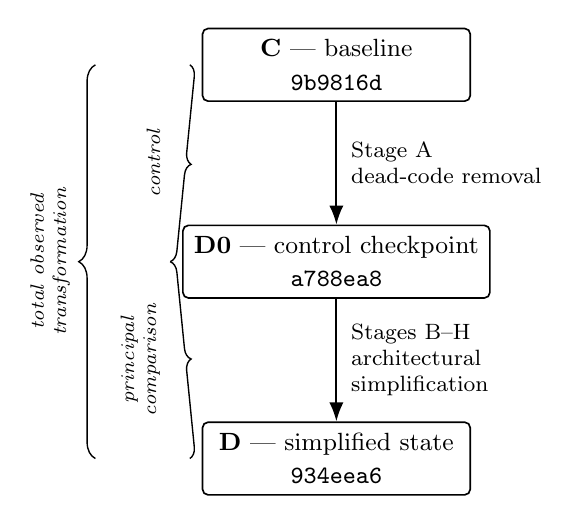
\begin{tikzpicture}[
  font=\small,
  mzstate/.style={draw,rounded corners=2pt,align=center,inner sep=4pt,
                minimum width=3.4cm,line width=0.6pt},
  mzflow/.style={-{Latex[length=2.4mm]},line width=0.7pt},
  mzlab/.style={align=left,font=\footnotesize,inner sep=2pt},
  mzrole/.style={align=center,font=\scriptsize\itshape,inner sep=1pt}
]

\node[mzstate] (C)  at (0,0)      {\textbf{C} --- baseline\\[1pt]\texttt{9b9816d}};
\node[mzstate] (D0) at (0,-2.5)   {\textbf{D0} --- control checkpoint\\[1pt]\texttt{a788ea8}};
\node[mzstate] (D)  at (0,-5.0)   {\textbf{D} --- simplified state\\[1pt]\texttt{934eea6}};

\draw[mzflow] (C)  -- node[mzlab,right=3pt] {Stage A\\dead-code removal} (D0);
\draw[mzflow] (D0) -- node[mzlab,right=3pt] {Stages B--H\\architectural\\simplification} (D);

%% comparison brackets on the left
\draw[decorate,decoration={brace,amplitude=4pt},line width=0.5pt]
  ($(C.west)+(-0.15,0)$) -- ($(D0.west)+(-0.15,0)$)
  node[mzrole,midway,left=6pt,rotate=90,anchor=south] {control};
\draw[decorate,decoration={brace,amplitude=4pt},line width=0.5pt]
  ($(D0.west)+(-0.15,0)$) -- ($(D.west)+(-0.15,0)$)
  node[mzrole,midway,left=6pt,rotate=90,anchor=south] {principal\\comparison};
\draw[decorate,decoration={brace,amplitude=6pt,mirror},line width=0.5pt]
  ($(C.west)+(-1.35,0)$) -- ($(D.west)+(-1.35,0)$)
  node[mzrole,midway,left=8pt,rotate=90,anchor=south] {total observed\\transformation};

\end{tikzpicture}
\caption{Experimental design. The same system is observed at three states
pinned to immutable commits. \textbf{D0 is a control checkpoint, not a third
competing architecture}: it isolates the effect of deleting unreachable code
from the effect of the architectural intervention, so that the principal
comparison D0~$\rightarrow$~D is not confounded by it. States C and D also
carry annotated tags, and each state has a frozen branch. The figure is
methodological: no quality indicator appears in it.}
\label{fig:design}
\end{figure}


Three snapshots of \texttt{Assets/Scripts} were defined, each pinned to an
immutable commit and recovered for measurement in an isolated worktree
(Figure~\ref{fig:design}). Each state additionally carries a frozen branch, and
C and D carry annotated tags, so that a state can be recovered by commit, by tag
or by branch and the three routes agree.

The three states support three comparisons:

\begin{itemize}\itemsep2pt
\item $\text{C} \rightarrow \text{D0}$ --- the effect of removing dead code (control);
\item $\text{D0} \rightarrow \text{D}$ --- the effect of the architectural intervention (principal comparison);
\item $\text{C} \rightarrow \text{D}$ --- the total observed transformation.
\end{itemize}

D0 is not a third competing architecture. It exists because an audit of the
baseline found that a substantial part of the Domain layer had no consumers.
Deleting unreachable code changes every aggregate mean, because the deleted
population is not a random sample of the system. Without D0, that change would
have been indistinguishable from the effect of the architectural work.

\subsection{Architectural Simplification Protocol}

The intervention was not the application of a target architectural style. An
initial hypothesis of migrating the system to Clean Architecture / Ports and
Adapters was formulated, audited against the baseline, and \emph{rejected before
any code was written}: state C already had a Unity-free domain layer, separated
Data, Domain and Presentation folders, and abstractions carrying concrete
responsibilities. The decision rule adopted instead was:

\begin{quote}
\emph{For each existing abstraction, identify the responsibility it performs in
the running system. Retain the abstraction if and only if that responsibility is
concrete and is not already discharged elsewhere.}
\end{quote}

Four outcomes were possible for each abstraction: REMOVE, MERGE, STRENGTHEN
(the abstraction is justified but bypassed in practice) and KEEP\@. KEEP decisions
were recorded with their evidence, on the same footing as changes, so that a
retention is reportable as a result rather than as the absence of one.

The intervention proceeded in eight stages (Table~\ref{tab:stages}). Each stage
was implemented in isolation, compiled, verified against the test suite, and
approved by a human reviewer before the next stage began. Stage A alone
produced D0; stages B through H produced D.

\begin{table}[!htbp]
\centering
\caption{Intervention stages. Stage A produced the control state D0; stages B\textendash{} H
produced the simplified state D.}\label{tab:stages}
\small
\begin{tabular}{cp{0.68\columnwidth}}
\toprule
\textbf{Stage} & \textbf{Intervention} \\
\midrule
A & Dead-code removal: 11 files, 20 types \\
B & Data layer: one DTO and four mappers removed; transformation localized in the repositories \\
C & Audio boundary adopted: 56 concrete accesses to engine singletons reduced to 0 \\
D & Partial explicit composition: three dead registrations removed; one presenter composed by constructor; service registry deliberately retained \\
E & Score multiplier consolidated into the domain scoring service \\
F & Indicator-reagent semantics given a single owner in the domain entity \\
G & View\,$\leftrightarrow$\,orchestrator cycles broken through two role contracts \\
H & Panel-reset duplication replaced by the existing collaborator \\
\bottomrule
\end{tabular}
\end{table}

Two constraints were imposed on the intervention and observed throughout. No
\texttt{MonoBehaviour} was renamed, moved between namespaces, or relocated in a
way that would invalidate an asset GUID, because that would silently break
scene serialization. And no global access mechanism was to be replaced by
another global access mechanism: a change that substitutes one ambient
singleton for another was not counted as simplification.

\subsection{Use of an LLM-Based Coding Assistant}\label{sec:llmuse}

The code changes constituting the intervention were implemented with the
assistance of an LLM-based coding agent (Claude Code, Anthropic), operating
inside the staged protocol described above: the agent proposed and applied
changes within one stage at a time, and every stage was reviewed and explicitly
approved by a human author, passed the functional-parity protocol described in
the next subsection, and was subject to the recorded prohibitions before the
next stage began. The responsibility assessments and retention decisions
reported in Section~\ref{sec:rq1} were made and recorded under the same human
gates. The measurement instrument and the analysis scripts were produced by the
same process; every reported value is re-derived mechanically from the frozen
per-type and per-member records by a versioned verification script, so no
reported number rests on unreviewed assistant output. LLM-assisted refactoring
is itself an emerging research subject~\cite{yang2026}; here the assistant is
part of the intervention procedure, not an object of study, and the study makes
no claim about the effect of this assistance on productivity or on code
quality. Section~\ref{sec:threats} discusses it as a threat.

\subsection{Functional-Parity Protocol}

The experimental target was behavioural preservation between C and D for the
behaviour covered by the validation protocol. We do not claim, and did not
attempt to establish, formal functional equivalence between the two states;
what follows describes operationally what was verified and therefore the scope
of the preservation claim. Because the object is an engine-based game whose
wiring lives partly in serialized scene data, no single verification technique
is sufficient, so five were combined.

\emph{Behavioural characterization tests.} A baseline characterization suite of
\textbf{68 tests} was written against state C \emph{before} any modification, and
covered data loading and deserialization, solubility rules, gameplay rules,
session state, and the mapping behaviour of the data layer. That baseline was the
reference for the dead-code control: state D0 passed the same 68 tests, unchanged.

The suite then grew \emph{during} the intervention. Before or alongside each
stage that touched a behaviour not yet pinned down, tests were added to
characterize that behaviour first, so that the stage could be evaluated against
it: a nine-case deserialization spike and two further data-loading cases before
the DTO removal, repository materialization and entity invariant tests around the
mapper consolidation, score multiplier tests before the scoring change, and
indicator semantics tests before ownership of the reagent rule moved into the
domain. Tests introduced at a gate were retained in force for every subsequent
stage, unless the production abstraction they characterized had itself been
removed. Exactly one such retirement occurred: the thirteen mapping tests went
when the mapper types went, and their coverage was taken over by the repository
materialization and entity invariant tests written for the arrangement that
replaced them.

State D therefore ends with \textbf{118 tests passing}, of which \textbf{103 are
behavioural characterization tests} and \textbf{15 are architecture invariant
tests} (Table~\ref{tab:suite}). The 118/118 figure is evidence about the final
suite; it is not a claim that all 118 tests existed before the first change to C.

\emph{Architecture invariant tests.} Fifteen of the final tests do not exercise
behaviour at all. They scan the source of the measured tree and assert structural
properties --- that no call site outside the audio adapter reaches the engine
audio singletons directly, and that the view contracts carry no engine types.
These were introduced by the stages that established the properties they guard,
and they are reported separately because they are evidence of \emph{structural}
conformance and contribute nothing to the argument for behavioural preservation.

The behavioural suite compiles the engine-free production files outside Unity; it
is not part of the population measured by the instrument. It deliberately
preserves several behaviours that would ordinarily be treated as defects,
including a difficulty asset with a zero score multiplier, a divergence in the
default difficulty, an inert branch in a UI controller, and the specific parsing
policy applied to malformed dataset entries. Correcting any of them would have
changed behaviour and broken the preservation target.

\begin{table}[!htbp]
\centering
\caption{Growth of the validation suite. The baseline was written against C
before any modification; later tests were added by the stages that touched the
behaviour or property they characterize.}\label{tab:suite}
\small
\begin{tabular}{@{}p{0.58\columnwidth}r p{0.24\columnwidth}@{}}
\toprule
\textbf{Added} & \textbf{Tests} & \textbf{Kind} \\
\midrule
Baseline, against C            & 68  & behavioural \\
\quad \emph{unchanged through Stage A (D0)} & \emph{68} & \emph{behavioural} \\
\addlinespace
Deserialization spike, Stage B & 11  & behavioural \\
Repository materialization, Stage B & 14 & behavioural \\
Entity invariants, Stage B     & 5   & behavioural \\
\quad \emph{mapping tests retired with the mapper types} & \emph{$-13$} & \emph{behavioural} \\
Audio boundary, Stage C        & 9   & architecture invariant \\
Score multiplier, Stage E      & 8   & behavioural \\
Indicator semantics, Stage F   & 10  & behavioural \\
View boundary, Stage G         & 6   & architecture invariant \\
\midrule
\textbf{State D, final}        & \textbf{118} & \textbf{103 + 15} \\
\bottomrule
\end{tabular}
\end{table}

\emph{Compilation.} Both through an isolated project definition and through the
engine's own assembly, in each state.

\emph{Engine import.} The Unity project was imported in state D with zero
missing-script errors and zero serialization errors, confirming that no GUID or
serialized binding was invalidated.

\emph{Manual full-flow verification.} A scripted walkthrough of the complete
game flow in all three modes.

\emph{Smoke verification} after the final stage, covering phase restart, panel
reset and return to menu.

\subsection{Measurement Instrument}

All three states were measured with a single instrument, frozen at one commit
and never read from inside the measured worktrees. It consists of a Roslyn-based
metrics extractor built on \texttt{Microsoft.CodeAnalysis.CSharp} 4.11.0, plus
SonarAnalyzer.CSharp 10.31.0.145097 and the engine's own analyzers, executed with
the \texttt{dotnet} SDK 9.0.306 under Unity 6000.4.1f1. Each state is recovered with a detached
worktree at its pinned commit, so production content and measurement tooling
remain separate; no snapshot is modified to accommodate the instrument.

The instrument reports, per type, lines of code, an approximate efferent
coupling count defined below, and whether the type is engine-instantiated; and,
per member, cyclomatic complexity and maintainability index. Aggregations are
computed from the raw per-type and per-member records rather than from summary
output.

\medskip\noindent\textbf{Maintainability index.} The instrument computes the
Microsoft variant of the maintainability index~\cite{coleman1994}:
$\mathrm{MI} = \max\bigl(0,\ \tfrac{100}{171}(171 - 5.2\ln V - 0.23\,\mathrm{CC}
- 16.2\ln \mathrm{LOC})\bigr)$, where $V$ is Halstead volume --- clamped at zero,
rescaled to a 0--100 range, and without the comment-percentage term of the
original formulation. It is computed per member and aggregated as a mean.

\medskip\noindent\textbf{Engine dependency.} A type is counted as
engine-dependent when its declared base list contains \texttt{MonoBehaviour} or
\texttt{ScriptableObject} --- that is, when the type is one the engine itself
instantiates, serializes and drives through its lifecycle. The check is
syntactic and considers only the \emph{directly} declared base types.

\medskip\noindent\textbf{Approximate efferent coupling.} For each type the
instrument counts the distinct capitalised identifiers appearing anywhere inside
the type declaration. This approximates Martin's efferent coupling
\cite{martin2003} without resolving symbols, and we therefore report it as a
\emph{structural coupling proxy} rather than as $C_e$ itself. It over-counts,
because a capitalised identifier also matches an invoked method name, a
property, an enum member or a constant; and it under-counts dependencies
expressed without a capitalised identifier. Section~\ref{sec:threats} states the
consequences. We use it because it is stable across the three states and
computed identically for all of them, so differences remain comparable even
though the absolute level is not a count of depended-upon types.

Two properties of the instrument were verified explicitly.\ \emph{Determinism}:
re-executing the pipeline on state D produced byte-identical artefacts,
including the analyzer SARIF\@. \emph{Version equivalence}: an error in the
project-generation step was found and corrected during the study; after the
correction, state C was re-measured through the real entry point and the
resulting files were byte-identical to those produced before, so all three
states are measured by the same instrument version.

Analyzer violation counts were also collected (C 197, D0 191, D 143). They are
auxiliary pipeline output and are not used to answer any research question here;
interpreting individual findings belongs to a separate study.

\subsection{Component Classification}

To answer RQ3, every source file was assigned to exactly one category. The
assignment was derived mechanically from the commit history --- which files each
stage touched --- rather than from post-hoc judgement.

\begin{description}\itemsep2pt
\item[DEAD CODE REMOVED] Present in C, removed exclusively in $\text{C}\rightarrow\text{D0}$,
after triple evidence of unreachability: no C\# references, no GUID references in
scenes, prefabs or assets, and no occurrence of the type name in serialized YAML\@.
\item[DIRECTLY REFACTORED] Component whose code or responsibility was a deliberate
target of stages B\textendash{} H.
\item[INDIRECTLY AFFECTED] Component changed only to accommodate a change whose
primary target was another component.
\item[PRESERVED] Existing component deliberately left unmodified by the relevant
architectural interventions.
\item[NEW INTERVENTION ARTIFACT] Element absent from the baseline, introduced as a
necessary part of the intervention.
\end{description}

A component that does not exist in a given state is recorded as \emph{absent},
never as zero. A NEW INTERVENTION ARTIFACT therefore has no row for C or D0, and
DEAD CODE REMOVED has no row for D0 or D. Substituting zero would inject
artificial values into every mean.

These five labels map onto the four population roles that matter for the
analysis in Section~\ref{sec:rq2}: components \emph{removed} from the measured
population (DEAD CODE REMOVED), components \emph{added} to it (NEW INTERVENTION
ARTIFACT), components \emph{modified} while remaining in it (DIRECTLY REFACTORED
and INDIRECTLY AFFECTED, kept apart because the first were deliberate targets and
the second were not), and components \emph{preserved} unchanged (PRESERVED). We
use the five-label form throughout, because it is the form recorded in the
analysis scripts and in the replication package; renaming it in the manuscript
alone would break that correspondence.

\subsection{Analysis Procedure}

Three analyses were performed on the frozen measurements.

\emph{Aggregate comparison.} All summary values were recomputed from the raw
per-type and per-member records in each state and cross-checked against the
instrument's own summary. All 48 values --- 16 indicators across three states ---
matched.

\emph{Matched-population analysis.} Aggregate means confound two phenomena:
change inside surviving components, and change in the population being averaged.
Components were therefore matched across states by a stable identity key ---
\texttt{file|type} for types and \texttt{file|type|member} for members --- and
the mean was recomputed over the intersection only. Keys that were not unique
within a state, which occurred for two method overloads in each state, were
\emph{excluded} from matching rather than resolved by assumption.

\emph{Category analysis.} Metrics were aggregated within each RQ3 category, with
units kept explicit: lines of code, approximate efferent coupling and type counts are
per-type quantities; cyclomatic complexity and maintainability index are
per-member quantities, and group-level values for them are means over the
members belonging to the group, never aggregated per type.

Inferential significance testing was not used, because the study observes the
complete measured component population of a single system at fixed states and
does not posit a sampling model that would justify such inference. All reported
quantities are descriptive, and no test is reported.

\medskip\noindent\textbf{Chain of evidence.} Every quantitative statement in
Section~\ref{sec:results} can be traced backwards through a fixed path: from the
reported value, to the aggregation script, to the per-type or per-member record
in the frozen result set, to the state's pinned commit, to the source file it was
computed from. Every architectural statement traces from the claim, to the row of
Table~\ref{tab:rq1}, to the audit record holding that concern's evidence and
decision, to the stage commit that implemented it --- or, for a retention, to the
recorded rationale for not changing anything. The RQ3 category of a file is
determined by which stage commits touched it, whereas its metrics are computed
from the measured source states, so the two are read from \emph{distinct}
artefacts. They are not independent in a statistical or causal sense: both
ultimately derive from the same source changes, which is why
Section~\ref{sec:rq3} states the circularity in the containment result rather
than treating the classification as externally validated.


%% =========================================================================
\section{Results}\label{sec:results}
%% =========================================================================

\subsection{RQ1 --- Architectural Reorganization}\label{sec:rq1}

\begin{figure}[!htbp]
\centering
\resizebox{\textwidth}{!}{%
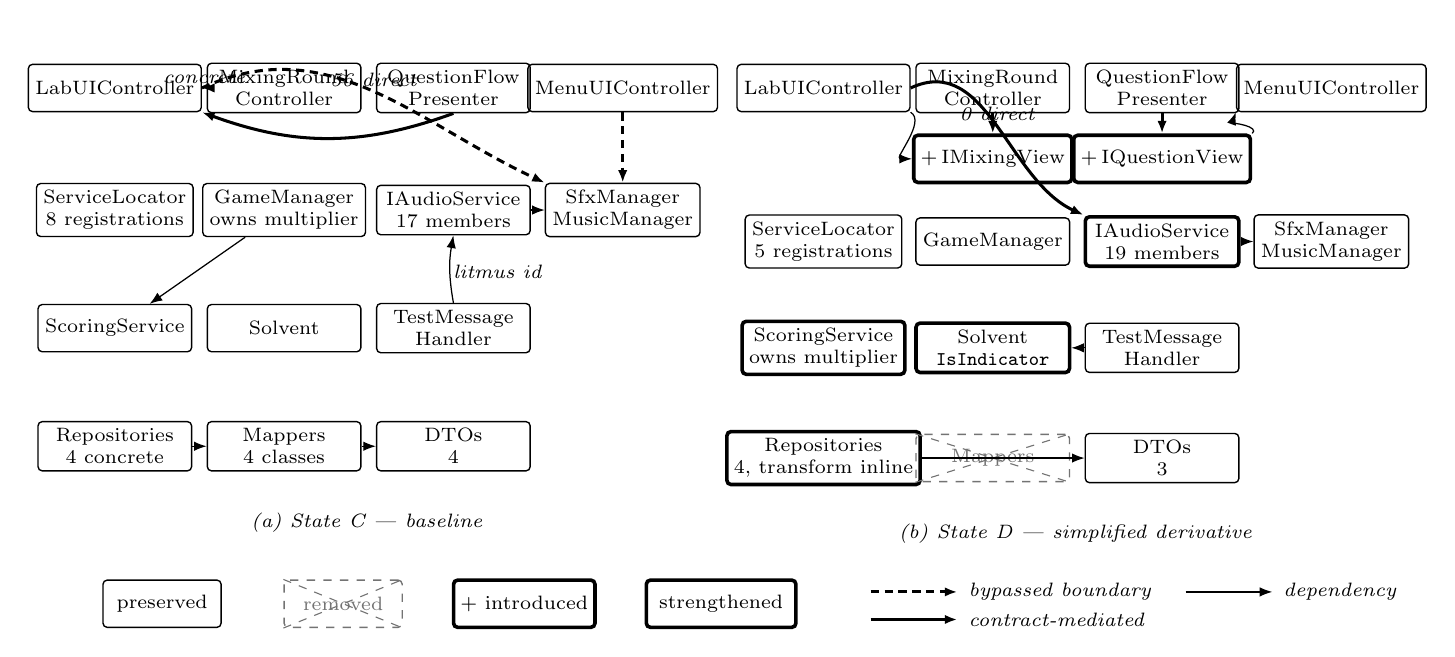
\begin{tikzpicture}[
  font=\scriptsize,
  mzband/.style={draw,dashed,rounded corners=3pt,inner sep=5pt,line width=0.4pt,
               draw=black!45},
  bandmzlab/.style={font=\scriptsize\bfseries,anchor=west,inner sep=1pt},
  mzcomp/.style={draw,rounded corners=1.5pt,align=center,inner sep=2.5pt,
               minimum height=6mm,minimum width=1.95cm,line width=0.5pt},
  mzgone/.style={mzcomp,dashed,draw=black!55,text=black!55,line width=0.5pt},
  mznew/.style={mzcomp,line width=1.3pt},
  mzstrong/.style={mzcomp,line width=1.3pt},
  mzdep/.style={-{Latex[length=1.6mm]},line width=0.45pt},
  mzbypass/.style={-{Latex[length=1.6mm]},line width=1.1pt,densely dashed},
  mzfixed/.style={-{Latex[length=1.6mm]},line width=1.1pt},
  mznote/.style={font=\scriptsize\itshape,inner sep=1pt}
]

%% ============================ PANEL (a) STATE C =========================
\begin{scope}[shift={(0,0)}]
  \node[mzcomp] (aLab)  at (0.00,0)     {LabUIController};
  \node[mzcomp] (aMix)  at (2.15,0)     {MixingRound\\Controller};
  \node[mzcomp] (aQfp)  at (4.30,0)     {QuestionFlow\\Presenter};
  \node[mzcomp] (aMenu) at (6.45,0)     {MenuUIController};

  \node[mzcomp] (aSL)   at (0.00,-1.55) {ServiceLocator\\\scriptsize 8 registrations};
  \node[mzcomp] (aGM)   at (2.15,-1.55) {GameManager\\\scriptsize owns multiplier};
  \node[mzcomp] (aIA)   at (4.30,-1.55) {IAudioService\\\scriptsize 17 members};
  \node[mzcomp] (aSfx)  at (6.45,-1.55) {SfxManager\\MusicManager};

  \node[mzcomp] (aScr)  at (0.00,-3.05) {ScoringService};
  \node[mzcomp] (aSol)  at (2.15,-3.05) {Solvent};
  \node[mzcomp] (aTmh)  at (4.30,-3.05) {TestMessage\\Handler};

  \node[mzcomp] (aRep)  at (0.00,-4.55) {Repositories\\\scriptsize 4 concrete};
  \node[mzcomp] (aMap)  at (2.15,-4.55) {Mappers\\\scriptsize 4 classes};
  \node[mzcomp] (aDto)  at (4.30,-4.55) {DTOs\\\scriptsize 4};

  \draw[mzfixed]  (aMix) -- node[mznote,above,pos=0.5] {concrete} (aLab);
  \draw[mzfixed]  (aQfp.south) to[out=200,in=340] (aLab.south east);
  \draw[mzbypass] (aLab.east)  to[out=25,in=155] node[mznote,above] {56 direct} (aSfx.north west);
  \draw[mzbypass] (aMenu) -- (aSfx);
  \draw[mzdep]    (aIA) -- (aSfx);
  \draw[mzdep]    (aRep) -- (aMap);
  \draw[mzdep]    (aMap) -- (aDto);
  \draw[mzdep]    (aGM) -- (aScr);
  \draw[mzdep]    (aTmh.north) to[out=100,in=260] node[mznote,right,pos=0.45] {litmus id} (aIA.south);

  \node[mznote,anchor=north] at (3.2,-5.35) {(a) State C --- baseline};
\end{scope}

%% ============================ PANEL (b) STATE D =========================
\begin{scope}[shift={(9.0,0)}]
  \node[mzcomp] (bLab)  at (0.00,0)     {LabUIController};
  \node[mzcomp] (bMix)  at (2.15,0)     {MixingRound\\Controller};
  \node[mzcomp] (bQfp)  at (4.30,0)     {QuestionFlow\\Presenter};
  \node[mzcomp] (bMenu) at (6.45,0)     {MenuUIController};

  \node[mznew] (bIMV)  at (2.15,-0.90) {$+$\,IMixingView};
  \node[mznew] (bIQV)  at (4.30,-0.90) {$+$\,IQuestionView};

  \node[mzcomp]   (bSL)  at (0.00,-1.95) {ServiceLocator\\\scriptsize 5 registrations};
  \node[mzcomp]   (bGM)  at (2.15,-1.95) {GameManager};
  \node[mzstrong] (bIA)  at (4.30,-1.95) {IAudioService\\\scriptsize 19 members};
  \node[mzcomp]   (bSfx) at (6.45,-1.95) {SfxManager\\MusicManager};

  \node[mzstrong] (bScr) at (0.00,-3.30) {ScoringService\\\scriptsize owns multiplier};
  \node[mzstrong] (bSol) at (2.15,-3.30) {Solvent\\\scriptsize \texttt{IsIndicator}};
  \node[mzcomp]   (bTmh) at (4.30,-3.30) {TestMessage\\Handler};

  \node[mzstrong] (bRep) at (0.00,-4.70) {Repositories\\\scriptsize 4, transform inline};
  \node[mzgone]   (bMap) at (2.15,-4.70) {Mappers};
  \node[mzcomp]   (bDto) at (4.30,-4.70) {DTOs\\\scriptsize 3};

  \draw[dashed,draw=black!55] (bMap.north west) -- (bMap.south east);
  \draw[dashed,draw=black!55] (bMap.south west) -- (bMap.north east);

  \draw[mzfixed] (bMix) -- (bIMV);
  \draw[mzfixed] (bQfp) -- (bIQV);
  \draw[mzdep]   (bLab.south east) to[out=330,in=180] (bIMV.west);
  \draw[mzdep]   (bIQV.north east) to[out=40,in=250] (bMenu.south west);
  \draw[mzfixed] (bLab.east) to[out=25,in=155] node[mznote,above] {0 direct} (bIA.north west);
  \draw[mzdep]   (bIA) -- (bSfx);
  \draw[mzdep]   (bRep) -- (bDto);
  \draw[mzdep]   (bTmh) -- (bSol);

  \node[mznote,anchor=north] at (3.2,-5.50) {(b) State D --- simplified derivative};
\end{scope}

%% ================================ LEGEND ================================
\begin{scope}[shift={(0,-6.55)}]
  \node[mzcomp,minimum width=1.5cm] (lp) at (0.6,0) {preserved};
  \node[mzgone,minimum width=1.5cm] (lr) at (2.9,0) {removed};
  \node[mznew,minimum width=1.5cm] (ln) at (5.2,0) {$+$ introduced};
  \node[mzstrong,minimum width=1.9cm] (ls) at (7.7,0) {strengthened};
  \draw[dashed,draw=black!55] (lr.north west) -- (lr.south east);
  \draw[dashed,draw=black!55] (lr.south west) -- (lr.north east);
  \draw[mzbypass] (9.6,0.15) -- (10.7,0.15); \node[mznote,anchor=west] at (10.8,0.15) {bypassed boundary};
  \draw[mzfixed]  (9.6,-0.2) -- (10.7,-0.2); \node[mznote,anchor=west] at (10.8,-0.2) {contract-mediated};
  \draw[mzdep]    (13.6,0.15) -- (14.7,0.15); \node[mznote,anchor=west] at (14.8,0.15) {dependency};
\end{scope}

\end{tikzpicture}}

\caption{Architectural component and dependency view of the two states, drawn
at the same level of abstraction and with preserved components in the same
positions so that the panels can be read against each other. State D is a
simplified derivative of the baseline, not a different architectural family:
most components are preserved, four mapper classes and one DTO are removed,
two role contracts are introduced, and three boundaries are strengthened.
Encoding does not rely on colour: preserved components have a plain border,
removed ones a dashed border with a cross, introduced ones a heavy border with
a $+$, and strengthened ones a heavy border. Every element and edge shown was
verified against the pinned snapshots.}
\label{fig:arch}
\end{figure}


Figure~\ref{fig:arch} shows what changed structurally between the two states,
and Table~\ref{tab:rq1} records the reasoning behind each change and each
retention. The figure answers \emph{what} moved; the table answers \emph{why}.

Table~\ref{tab:rq1} records the outcome of the responsibility assessment for
each abstraction examined. Thirteen concerns were audited: three led to removal or
merging, two to strengthening, three to a local simplification or a change
of ownership, and five to a documented retention.

\begingroup
\footnotesize
\setlength{\tabcolsep}{4pt}
\begin{longtable}{p{0.15\textwidth}p{0.13\textwidth}p{0.31\textwidth}p{0.14\textwidth}p{0.15\textwidth}}
\caption{RQ1 --- responsibility assessment of each abstraction. Retention
decisions are reported with the same status as changes.}\label{tab:rq1}\\
\toprule
\textbf{Concern} & \textbf{Initial hypothesis} & \textbf{Evidence found} & \textbf{Decision} & \textbf{Consequence} \\
\midrule
\endfirsthead
\toprule
\textbf{Concern} & \textbf{Initial hypothesis} & \textbf{Evidence found} & \textbf{Decision} & \textbf{Consequence} \\
\midrule
\endhead
\bottomrule
\endlastfoot
\texttt{QuestionMapper} & Redundant & Purely positional pass-through; invariants live in the entity & REMOVE & Binding now rests on constructor parameter names \\
\addlinespace
\texttt{QuestionDto} & Redundant & 1:1 copy, no type conversion & REMOVE & Verified by a nine-criterion spike before removal \\
\addlinespace
\texttt{CompoundMapper}, \texttt{SolventMapper}, \texttt{SolutionMapper} & Duplicated & One caller each; real conversion present & MERGE & Transformation became a private repository method \\
\addlinespace
Remaining three DTOs & Useful & Case conversion, string-to-enum, one rename & KEEP & Representation boundary preserved \\
\addlinespace
\texttt{Json*Repository} public surface & Cleanup candidate & Four methods without consumers, three of which lost them \emph{in Stage A} & KEEP & Removing them would credit the intervention with a control effect \\
\addlinespace
\texttt{IAudioService} & Necessary but bypassed & 56 concrete accesses against 2 port consumers & STRENGTHEN & 56 $\rightarrow$ 0; port gained two availability members \\
\addlinespace
\texttt{ServiceLocator} & \textbf{Redundant} & Full removal would require scene scanning, layer inversion or a lifetime change & \textbf{HYPOTHESIS REJECTED} $\rightarrow$ KEEP + SIMPLIFY & Three dead registrations removed; registry retained for cross-scene lifetime \\
\addlinespace
\texttt{GameManager} responsibilities & Broad decomposition & Only scoring was split across layers & Selective SIMPLIFY & One move, seven documented retentions \\
\addlinespace
Litmus indicator semantics & Duplicated in Presentation & Confirmed at two sites & MOVE & Ownership moved to \texttt{Solvent.\allowbreak{}IsIndicator} \\
\addlinespace
\texttt{TreeSolvent\allowbreak{}GroupButtons} & Duplicated & The consumer sustaining the duplication was removed \emph{in Stage A} & \textbf{HYPOTHESIS REJECTED} $\rightarrow$ KEEP & Content is editorial and carries markup \\
\addlinespace
View\,$\leftrightarrow$\,orchestrator cycles & Breakable & Two concrete reverse dependencies, two engine-type leaks & STRENGTHEN & \texttt{IMixingView} and \texttt{IQuestionView} introduced; \texttt{ILabView} untouched \\
\addlinespace
God-object candidates & Decomposition & Only one duplication had a better existing owner & Local SIMPLIFY & One consolidation, nine retentions \\
\addlinespace
Pre-existing dead members & Dead & Already dead in C & PRESERVE FOR PARITY & Retained so control and intervention stay separable \\
\end{longtable}
\endgroup


\medskip\noindent\textbf{Simplification did not mean minimising abstractions.}
Structurally, the system that followed the intervention had \emph{fewer classes
and more interfaces}: from D0 to D the class count fell from 65 to 60, the
interface count rose from 12 to 14, and the member count rose from 451 to 457. Five files
were removed and two were added.

This is the opposite of the shape usually associated with simplification, and it
is a direct consequence of the decision rule rather than an anomaly. The rule was
not ``reduce the number of abstractions''; it was ``retain an abstraction exactly
when it carries a concrete responsibility''. Applied consistently, that rule
moves in both directions at once, and the four decisions that most clearly show
it are:

\begin{itemize}\itemsep2pt
\item \texttt{QuestionMapper} --- \textbf{removed}: it performed a positional
copy the entity constructor already performed.
\item \texttt{IAudioService} --- \textbf{strengthened}: the responsibility was
real, but 56 call sites bypassed it; the port gained two members and the bypasses
went to zero.
\item \texttt{ServiceLocator} --- \textbf{retained and simplified}: the removal
attempt revealed a cross-scene lifetime responsibility nothing else discharged;
three dead registrations were removed and the registry kept.
\item \texttt{IMixingView} and \texttt{IQuestionView} --- \textbf{introduced}:
a responsibility existed --- decoupling two views from their orchestrators --- that
no abstraction expressed.
\end{itemize}

We therefore do not report abstraction count as a measure of simplification, and
a reader should not infer from the interface count that the system became more
elaborate. What changed is which abstractions exist, not how many.

\medskip\noindent\textbf{Four mechanisms of abstraction utility.} Looked at
again, those four decisions are not four instances of one rule. They are four
different reasons an abstraction can or cannot be justified, and the difference
matters for how a candidate should be assessed:

\begin{enumerate}\itemsep2pt
\item \emph{No current responsibility} (\texttt{QuestionMapper}) --- removed.
Decidable by reading the source.
\item \emph{A concrete responsibility, bypassed in practice}
(\texttt{IAudioService}) --- strengthened. Also decidable by reading the source,
provided one counts call sites rather than inspecting the abstraction alone.
\item \emph{A responsibility only the removal attempt revealed}
(\texttt{ServiceLocator}) --- retained. \emph{Not} decidable by reading the
source: the responsibility lived in the runtime composition model, which for an
engine-based system is partly held in serialized scene data.
\item \emph{A justification an earlier stage had already removed}
(\texttt{TreeSolventGroupButtons}) --- retained. Decidable when first assessed,
and wrong by the time it was acted on.
\end{enumerate}

Cases 3 and 4 both end in a retained abstraction, and it would be convenient to
file both as false positives of the audit. That would lose the distinction that
matters: in case 3 the analysis was incomplete, whereas in case 4 the analysis
was correct and the system moved underneath it. The first argues for attempting
a removal before trusting a static verdict; the second argues for re-deriving
the candidate list after each stage rather than fixing it at the outset.

\subsection{RQ2 --- Internal Quality Indicators}\label{sec:rq2}

\subsubsection{Aggregate measurements}

Table~\ref{tab:aggregate} reports the full aggregate profile of the three
states.

\begin{table}[!htbp]
\centering
\caption{Aggregate measurements across the three states. CC and MI are
per-member quantities; LOC, coupling and type counts are per-type.}\label{tab:aggregate}
\small
\begin{tabular}{lrrr}
\toprule
\textbf{Indicator} & \textbf{C} & \textbf{D0} & \textbf{D} \\
\midrule
Source files            & 91    & 80    & 77 \\
LOC (non-blank)         & 5\,093 & 4\,738 & 4\,729 \\
Comment lines           & 695   & 649   & 825 \\
Classes                 & 79    & 65    & 60 \\
Interfaces              & 16    & 12    & 14 \\
Structs / records       & 7     & 5     & 5 \\
Enums                   & 9     & 9     & 9 \\
Members                 & 496   & 451   & 457 \\
\addlinespace
CC mean                 & 2.33  & 2.39  & 2.38 \\
CC median               & 2.0   & 2.0   & 2.0 \\
CC max                  & 17    & 17    & 17 \\
CC total                & 1\,158 & 1\,078 & 1\,089 \\
\addlinespace
MI mean                 & 72.5  & 71.7  & 71.8 \\
MI median               & 71.2  & 70.2  & 70.9 \\
Members with MI $\geq$ 65 & 323 & 287   & 293 \\
\quad as \% of members   & 65.1  & 63.6  & 64.1 \\
Members with CC $>$ 10   & 6     & 6     & 5 \\
\addlinespace
Approx. efferent coupling & 11.4 & 12.8  & 13.4 \\
Engine-coupled classes  & 24    & 23    & 23 \\
\quad as \% of classes  & 30.4  & 35.4  & 38.3 \\
\bottomrule
\end{tabular}
\end{table}

Between D0 and D the system lost 3 files, 9 lines of code and 5 classes, and
gained 2 interfaces and 6 members. The three principal indicators moved very
little: MI mean rose by 0.1 on a 0--100 scale, CC mean fell by 0.01 on a scale
whose observed mean is about 2.4, and the mean coupling proxy rose by 0.6.

Between C and D0 --- the control --- MI mean fell by 0.8 and mean efferent
coupling rose by 1.4, even though the only action taken was the deletion of
unreachable code. Figure~\ref{fig:trajectories} plots the three principal
indicators across the three states: in each panel the control step moves the
mean more than the intervention step does.

\begin{figure}[!htbp]
\centering
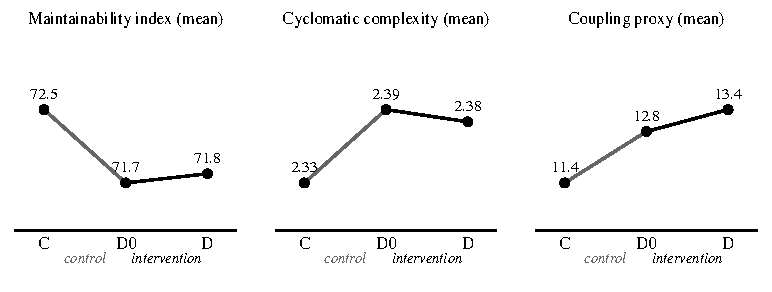
\includegraphics{fig-trajectories.pdf}
\caption{Aggregate trajectories of the three principal indicators across the
states (values from Table~\ref{tab:aggregate}). The C\,$\rightarrow$\,D0
segment is the control --- dead-code removal only --- and the
D0\,$\rightarrow$\,D segment is the architectural intervention. The control
step moves every mean more than the intervention step.}\label{fig:trajectories}
\end{figure}

\subsubsection{Matched-population analysis}

The aggregate figures above mix two phenomena: change inside components that
exist in both states, and change in the population over which the mean is taken.
Table~\ref{tab:matched} separates them.

\begin{table}[!htbp]
\centering
\caption{Matched-population analysis, D0 $\rightarrow$ D. Holding the population
fixed reverses the direction of the system-wide MI and CC movement; the matched
members themselves also change, by small amounts.}\label{tab:matched}
\small
\begin{tabular}{lrrr}
\toprule
\textbf{Basis} & \textbf{D0} & \textbf{D} & \textbf{$\Delta$} \\
\midrule
\multicolumn{4}{l}{\emph{Members, system-wide (n = 442 matched)}} \\
MI, aggregate mean      & 71.7  & 71.8  & $+0.1$ \\
MI, matched members     & 71.87 & 71.80 & $-0.06$ \\
CC, aggregate mean      & 2.39  & 2.38  & $-0.01$ \\
CC, matched members     & 2.41  & 2.42  & $+0.01$ \\
\addlinespace
\multicolumn{4}{l}{\emph{Directly refactored types}} \\
Coupling, matched (n = 19) & 26.84 & 28.37 & $+1.53$ \\
Coupling, raw group mean   & 22.29 & 28.37 & $+6.08$ \\
Coupling of removed types  & 5.00  & ---   & --- \\
\bottomrule
\end{tabular}
\end{table}

\begin{figure}[!htbp]
\centering
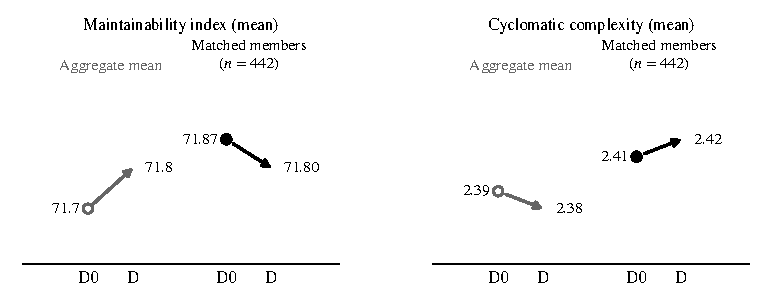
\includegraphics{fig-matched.pdf}
\caption{Aggregate versus matched-population movement of the two per-member
indicators, D0\,$\rightarrow$\,D (values as printed in
Table~\ref{tab:matched}). Holding the population fixed (black) reverses the
direction that the aggregate mean (grey) reports for both indicators.}\label{fig:matched}
\end{figure}

Three observations follow.

\emph{First, the direction reverses} (Figure~\ref{fig:matched}). The aggregate MI mean rises while
matched-member MI falls; the aggregate CC mean falls while matched-member CC
rises. Two phenomena are present at once, and neither is absent. Population
composition --- the eleven new members, largely simple properties scoring high on
MI, and the five removed ones --- reversed the direction of the aggregate signal.
At the same time the surviving members did change, by $-0.06$ on MI and $+0.01$ on
CC\@. The correct statement is therefore that composition reversed the direction of
the aggregate movement, while the change among surviving members was small and
opposite in direction to it --- not that the surviving code was unchanged.
Reporting the aggregate delta alone would have supported the statement that
maintainability improved slightly; the matched analysis does not support that
reading.

\emph{Second, the magnitudes are small in absolute terms.} Only 65 of 442 matched
members (14.7\%) changed MI at all, and only 12 (2.7\%) changed CC\@. The movements
are 0.06 on a 0--100 scale and 0.01 on a scale whose observed mean is about 2.4.
We do not infer practical significance from changes of this magnitude, in either
direction, and we did not adopt a threshold that would license such an
inference.

\emph{Third, the coupling increase is real and partly genuine.} Of the $+6.08$
raw increase in the directly refactored group, $+1.53$ is within-type change
among the 19 surviving types, and the remainder follows from removing five types
whose mean coupling (5.00) was far below the group mean. Fourteen of the 19
survivors changed, twelve upwards and two downwards; the largest increases were
in the repositories that absorbed the mapper logic --- one rose from 12 to 19,
another from 14 to 19, another from 12 to 15. Architectural responsibility
redistribution and measured coupling increase are related here, but they are not
the same phenomenon, and the increase is not merely a redistribution artefact.

\subsubsection{Engine dependency}

The set of engine-instantiated types --- those directly declaring
\texttt{MonoBehaviour} or \texttt{ScriptableObject} as a base type --- was
compared by identity, not by count:

\begin{center}\small
\begin{tabular}{lr}
Engine-coupled types in D0 & 23 \\
Engine-coupled types in D  & 23 \\
Intersection               & 23 \\
Present only in D0         & --- (empty) \\
Present only in D          & --- (empty) \\
\end{tabular}
\end{center}

The set is identical. The percentage rose from 35.4\% to 38.3\% because the
class population fell from 65 to 60 while the absolute count stayed constant.
The percentage remains an accurate description of each state's composition; what
it does not indicate is that any type entered the engine-coupled set, since that
set was the same in D0 and D.

This is the clearest single result of the study, and it contradicted an
expectation that had been central to the earlier framing of the work.
Section~\ref{sec:discussion} examines what this indicator does and does not
capture. Here we report only that the set of types directly extending
\texttt{MonoBehaviour} or \texttt{ScriptableObject} was the same in both states,
and that the movement of the percentage is accounted for by the change in the
class population.

\subsection{RQ3 --- Distribution Across Component Categories}\label{sec:rq3}

Table~\ref{tab:rq3dist} gives the distribution of files across the five
categories in each state, and Table~\ref{tab:rq3metrics} the group metrics.

\begin{table}[!htbp]
\centering
\caption{RQ3 --- distribution of source files by category. A dash denotes
absence, not zero.}\label{tab:rq3dist}
\small
\begin{tabular}{lrrr}
\toprule
\textbf{Category} & \textbf{C} & \textbf{D0} & \textbf{D} \\
\midrule
Directly refactored        & 24 & 24 & 19 \\
Indirectly affected        & 1  & 1  & 1 \\
Preserved                  & 55 & 55 & 55 \\
Dead code removed          & 11 & ---& --- \\
New intervention artifact  & ---& ---& 2 \\
\midrule
\textbf{Total}             & \textbf{91} & \textbf{80} & \textbf{77} \\
\bottomrule
\end{tabular}
\end{table}

\begin{table}[!htbp]
\centering
\caption{RQ3 --- group metrics. The upper block is the intervention
(D0 $\rightarrow$ D); the lower block is the control (C $\rightarrow$ D0).}\label{tab:rq3metrics}
\footnotesize
\setlength{\tabcolsep}{2pt}
\begin{tabular}{lrrrrrrr}
\toprule
\textbf{Group} & \textbf{Types} & \textbf{Members} & \textbf{LOC} & \textbf{CC mean} & \textbf{MI mean} & \textbf{Coupling mean} & \textbf{Engine} \\
\midrule
Directly refactored, D0   & 24 & 199 & 2\,357 & 2.44 & 71.2 & 22.29 & 8 \\
Directly refactored, D    & 19 & 204 & 2\,505 & 2.43 & 71.4 & 28.37 & 8 \\
\addlinespace
Indirectly affected, D0   & 3  & 11  & 58    & 1.36 & 83.5 & 7.00  & 0 \\
Indirectly affected, D    & 3  & 12  & 67    & 1.33 & 84.0 & 7.67  & 0 \\
\addlinespace
\textbf{Preserved, D0}    & \textbf{64} & \textbf{241} & \textbf{3\,286} & \textbf{2.40} & \textbf{71.5} & \textbf{9.56} & \textbf{15} \\
\textbf{Preserved, D}     & \textbf{64} & \textbf{241} & \textbf{3\,286} & \textbf{2.40} & \textbf{71.5} & \textbf{9.56} & \textbf{15} \\
\addlinespace
New intervention artifact, D & 2 & 0 & 30 & n/a & n/a & 0.50 & 0 \\
\midrule
\multicolumn{8}{l}{\emph{Control, C $\rightarrow$ D0}} \\
Dead code removed (C only) & 20 & 45  & 356 & \textbf{1.78} & \textbf{80.3} & \textbf{4.50} & --- \\
Whole project in C & 111 & 496 & --- & 2.33 & 72.5 & 11.4 & --- \\
\bottomrule
\end{tabular}
\end{table}

The new intervention artifacts have zero members because both are pure
interfaces; the instrument assigns no cyclomatic complexity or maintainability
index to declarations without bodies. Their coupling of 0.50 is reported as
measured.

\begin{figure}[!htbp]
\centering
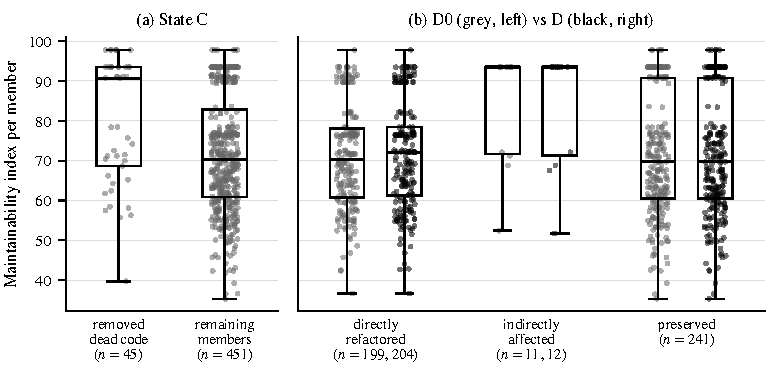
\includegraphics{fig-rq3.pdf}
\caption{Per-member maintainability-index distributions underlying
Table~\ref{tab:rq3metrics} (boxes: quartiles and median; points: individual
members). Panel (a): in state C, the members of the code removed as dead sit
visibly above the rest of the system. Panel (b): per category, D0 (grey, left)
against D (black, right); the preserved group is identical by construction,
and the directly refactored group changes only slightly. The new intervention
artifacts contribute no measured members and are omitted.}\label{fig:rq3}
\end{figure}

\medskip\noindent\textbf{The preserved group is metric-identical.} Across
D0~$\rightarrow$~D, the 64 preserved types show no change in any reported
indicator: same type count, same member count, same lines of code, same
complexity, same maintainability, same coupling, same engine-coupled count. In
the remaining groups the control transition C~$\rightarrow$~D0 is likewise near
zero: $-7$ lines and $-0.12$ coupling in the directly refactored group, $-0.02$
coupling in the preserved group, and no change at all in the indirectly affected
group.

\medskip\noindent\textbf{The removed dead code was not representative}
(Figure~\ref{fig:rq3}a). The 20
types deleted in the control had mean MI 80.3 against 72.5 for the project, mean
cyclomatic complexity 1.78 against 2.33, and a mean coupling proxy of 4.50
against 11.4. They were smaller, less complex and less coupled than the system
average --- which is unsurprising, since code that nothing calls tends to be
small and to depend on little. Removing them therefore changed the composition of
the population over which every mean is taken, and each aggregate mean moved in
the less favourable direction as a result. That movement is a property of the
subset removed, not a statement about the quality of the code that remained. This
is the confound the control state was introduced to isolate, and it is quantitatively large enough to have swamped the effect of the
architectural intervention had the two been measured together.

\medskip\noindent\textbf{Interpretation and its limit.} The measured structural
changes fall outside the source-preserved group, which remained
metric-identical, and inside the groups classified as directly or indirectly
affected. This is evidence that the changes were \emph{contained}. It is not an independent validation of
the classification and not a causal attribution: the preserved group is
\emph{defined} by the absence of relevant source changes, and the metrics are
derived from static code, so its metric identity partly follows from its
definition. Classification and result are not independent, and we do not claim
they are.

\subsection{Summary of Unexpected Findings}

Six results ran against the expectations held at the start of the study.

\begin{enumerate}\itemsep2pt
\item Removing dead code changed the composition of the measured population and
moved every normalized aggregate mean in the less favourable direction, because
the removed subset scored above the system average on every indicator.
\item Engine dependency did not fall: the same 23 types in D0 and D, with the
percentage rising through denominator change alone.
\item Simplification was accompanied by fewer classes but \emph{more} interfaces
and more members.
\item Two a-priori simplification hypotheses were rejected by implementation
evidence, for two different reasons.
\item The MI and CC movements reverse direction under matched-population
analysis, although all magnitudes are small.
\item Coupling rose in the repositories that absorbed the mapper logic, both by
redistribution and as a genuine within-type increase.
\end{enumerate}


%% Every Results float must be printed before the interpretation starts.
\FloatBarrier

%% =========================================================================
\section{Discussion}\label{sec:discussion}
%% =========================================================================

\subsection{Aggregate Indicators and Population Change}

The clearest methodological lesson of this study is that an aggregate mean over
a population that is itself being modified is a poor instrument for evaluating
an intervention that modifies the population.

Two of our three principal indicators change direction between the aggregate and
the matched view (Table~\ref{tab:matched}). Had we reported only the aggregate,
the natural narrative would have been that simplification produced a small
improvement in maintainability and a small reduction in complexity. The matched
analysis shows something different on two counts at once: within the 442 members
present in both states, maintainability moved down by 0.06 and complexity up by
0.01, and the aggregate signal was pulled the other way by eleven newly
introduced members, mostly simple properties that score well on MI\@. The
surviving code did change; what the composition of the population did was
reverse the direction the aggregate reported.

Both readings are arithmetically correct. They answer different questions. The
aggregate answers ``what is the profile of the system that now exists''; the
matched analysis answers ``what happened to the code that survived''. For
evaluating an intervention, the second is the relevant one, and it is the one
the literature reports less often. The aggregation literature has long warned
that the operator chosen over skewed metric distributions can change the
conclusion~\cite{vasilescu2011,mordal2013}; the population effect observed here
is the complementary hazard, produced not by the operator but by the
intervention silently redefining the set being operated on.

The same point applies with more force to the control transition, and there it
applies cleanly. Removing unreachable code is uncontroversially good practice~\cite{romano2020,eder2012}, and it moved every normalized indicator in this
system in the less favourable direction. In that transition no surviving code was
edited at all, so the entire movement is attributable to the change in the
population being averaged. A study that
combined dead-code removal with an architectural intervention and reported the
aggregate delta would have attributed this movement to the architecture.

This is consistent with, and gives a concrete mechanism for, the repeatedly
reported finding that refactoring produces mixed rather than uniform metric
outcomes~\cite{szoke2017,bavota2015,palomba2018}. Part of the mixture may be
population effects rather than disagreement about the value of the
transformations.

\subsection{What the Engine-Dependency Indicator Captures}

The engine-coupled set was identical in the D0 and D states: the same 23 types, with empty
differences in both directions. This is the result that most directly
contradicted the study's initial framing.

Interpreting this result requires being precise about what the indicator
measures. Our engine-dependency indicator counts types that directly declare
\texttt{MonoBehaviour} or \texttt{ScriptableObject} as a base type: the types
the engine itself instantiates and drives. That is one operational manifestation
of engine dependence, not a complete characterization of it. A type can use
\texttt{UnityEngine} APIs extensively --- for vectors, coroutines, resource
loading or scene management --- without extending either base class, and such a
type is not counted here. In state C, thirteen types reference
\texttt{UnityEngine} without being engine-instantiated; in state D, twelve. A
system can likewise depend on an engine through its lifecycle assumptions, its
serialization model or its scene composition without that dependence appearing
in this count at all. Engine dependence is
architecturally consequential --- the engine architecture literature treats
coupling to the engine core as a first-order concern~\cite{politowski2025,ullmann2023} --- and the point here is not that it carries
no architectural meaning, but that our indicator captures only its explicit
structural facet and should not be read as a measure of architectural decoupling.

Within that facet, the reason the set did not move follows from how the engine
composes an application. A component a scene instantiates must be a
\texttt{MonoBehaviour}; a field the editor serializes must be visible to the
engine's serializer; a lifetime spanning scene loads must be managed by an engine
mechanism~\cite{unitydocs}. Our interventions redistributed responsibilities
among the layers above these obligations, and none of them changed which
components the engine must itself instantiate and wire. A different intervention
--- extracting engine-facing logic into engine-free collaborators, or changing the
scene composition --- might have moved the set. Ours did not attempt that, and
this study cannot say what such an intervention would have produced.

The reporting implication is narrower and firmer. Because the percentage form of
the indicator takes the class population as its denominator, it moves whenever
that population moves. Reading 35.4\% $\rightarrow$ 38.3\% as increased engine
dependence would be a denominator artefact, and reading a hypothetical downward
movement as reduced dependence would be equally unfounded. Where the population
changes, the set and its differences carry the information; the percentage does
not.

The reporting practice this suggests is correspondingly modest. For
interventions that change the class population, reporting the engine-coupled set
and its set difference alongside the percentage avoids denominator ambiguity: the
percentage still describes each state, but only the set difference answers
whether any component entered or left engine dependence.

\subsection{Responsibility as a Decision Rule}

The intervention did not apply a target architectural style, and the a-priori
hypothesis of migrating to Clean Architecture was rejected during the audit,
before any code was written, because the baseline already had a Unity-free
domain and abstractions carrying real responsibilities.

What replaced it --- assessing each abstraction against the responsibility it
concretely performs --- produced an outcome that no style-driven rule would have
produced. It removed a DTO and four mappers, but retained three other DTOs that
performed genuine representation conversion. It retained a service locator that
a style-driven rule would have eliminated, because the removal attempt revealed a
cross-scene lifetime responsibility that nothing else discharged. And it
\emph{introduced} two interfaces, because two concrete cycles existed for which
no abstraction expressed the responsibility.

The four mechanisms identified in Section~\ref{sec:rq1} suggest a practical
ordering. Mechanisms 1 and 2 --- no responsibility, and bypassed responsibility
--- are decidable by static inspection. Mechanisms 3 and 4 are not. Mechanism 3
(the responsibility that only the removal attempt reveals) means that static
inspection can be \emph{incomplete}: some responsibilities are visible only in
the runtime composition model, which for an engine-based system lives partly in
serialized data. Mechanism 4 (the justification that an earlier transformation
already removed) means that a correct analysis can become obsolete during a
staged intervention, which is an argument for re-deriving candidates after each
stage rather than fixing the plan at the outset.

This connects to the architectural technical debt literature~\cite{verdecchia2020,verdecchia2021}, which characterizes such debt as decisions
that were appropriate when taken and later became obstacles. Mechanism 4 is the
inverse-and-benign case: an item of apparent debt whose justification
disappeared, making the item harmless rather than harmful, and detectable only
by re-examination.

\subsection{What Simplification Cost and What It Bought}

The intervention did not buy a better metric profile. Within surviving code the
indicators were flat to marginally worse, and the mean coupling proxy rose both
in aggregate ($+0.6$) and among matched surviving types in the directly
refactored group ($+1.53$).

The coupling increase has a concrete cause. Removing four mappers moved their
transformation logic into the repositories that had called them, so those
repositories now depend on more types than before. Whether this is an
improvement is a design judgement, not a metric one: the system has fewer
indirection layers and fewer components to keep consistent, at the cost of
repositories that know more. The metric records the cost and is silent about the
benefit --- which is precisely the limitation that the multi-property
maintainability models were designed to address~\cite{heitlager2007,baggen2012},
and a reason not to treat a coupling mean as a verdict.

Sas and Avgeriou~\cite{sas2020} found that practitioners in the embedded systems
industry rarely monitor design-time qualities at all, and that trade-offs
involving them therefore remain implicit. Our case is the complementary
situation: the design-time indicators were monitored, closely and with a frozen
instrument, and the trade-off still did not resolve into a verdict, because the
indicators price the cost of concentrating dependencies without pricing the
benefit of removing an indirection layer. Monitoring is necessary for making such
a trade-off explicit; on this evidence it is not sufficient for deciding it.

What the intervention did produce is structural: 56 direct accesses to engine
audio singletons reduced to zero behind an existing port; two concrete cycles
between views and orchestrators replaced by role contracts; one duplicated
domain rule given a single owner; three dead service registrations removed. These
are changes in the dependency structure that the aggregate indicators do not
express, and reporting them requires the architectural narrative of
Section~\ref{sec:rq1} alongside the numbers.

We deliberately do not claim that state D is better than state D0. The study
measured what changed; whether the trade is worthwhile depends on which future
changes the system will actually face, and that is not observable from a static
snapshot.

\subsection{Implications}

For \emph{researchers}: interventions that change component population should
report matched-population results alongside aggregate ones, and should separate
deletion effects from restructuring effects. In this study the deletion effect
was larger than the restructuring effect on every aggregate indicator.

For \emph{practitioners} working on engine-based systems: where an intervention
changes the class population, tracking the engine-coupled set alongside the
percentage removes an ambiguity the percentage alone cannot resolve; and
abstractions
should be assessed against the responsibility they discharge in the composed,
running system --- not against the catalogued pattern they resemble in source~\cite{gamma1995}.

For both: a retention decision, recorded with its evidence, is a result. Five of the thirteen audited
concerns in this study ended in a retention decision, and two of those
overturned an a-priori hypothesis. A protocol that only records changes would have reported
none of it.


\FloatBarrier

%% =========================================================================
\section{Threats to Validity}\label{sec:threats}
%% =========================================================================

We follow the categories of Runeson and H\"ost~\cite{runeson2009}.

\medskip\noindent\textbf{Construct validity.} MI, cyclomatic complexity and our
approximate efferent coupling are structural proxies, not measurements of the
maintainability that developers experience. The critiques are well established: cyclomatic
complexity is substantially a proxy for size~\cite{shepperd1988}, and MI is a
composite calibrated on a corpus unlike ours that incorporates both~\cite{coleman1994,ardito2020}. We mitigate this by reporting the indicators
separately as well as together, by reporting medians alongside means, and by
never treating a movement in one of them as a statement about maintainability.
For the same reason we use the term \emph{internal software quality indicators}
throughout.

\emph{Approximate efferent coupling} is the weakest construct of the three. As
defined in Section~\ref{sec:design}, it counts distinct capitalised identifiers
within a type rather than resolved external types, so its absolute level is not
a count of dependencies and should not be read as one. It both over-counts
(invoked method names, properties, enum members and constants are matched) and
under-counts (dependencies expressed without a capitalised identifier are
missed). We use it comparatively only: the same rule is applied to all three
states, so a difference between states reflects a change in the measured text
even though the level does not translate into a dependency count. Any reading of
our coupling figures as $C_e$ values would be unwarranted.

\emph{Engine dependency} is defined operationally as the number of types whose
declared base list contains \texttt{MonoBehaviour} or \texttt{ScriptableObject}.
Two limitations follow. First, the check is \emph{syntactic}: base types are
matched as text, without resolving the inheritance graph. Second, it considers
only \emph{directly} declared base types, so a class extending an intermediate
class that itself extends \texttt{MonoBehaviour} would not be counted; no such
case was audited in this system, and we did not verify their absence
exhaustively. The indicator therefore measures engine instantiation
specifically, not engine API usage in general, and a system could reduce its
use of engine APIs considerably without moving this count. Its percentage form
uses classes as denominator and is sensitive to population change, which is why
we report the set identity rather than the percentage as the result.

\medskip\noindent\textbf{Internal validity.} The eight stages were applied
sequentially and may interact. The D0 checkpoint isolates dead-code removal from
the architectural intervention, but it does not isolate stages B through H from
one another. Two concrete interactions were in fact observed and are reported in
Table~\ref{tab:rq1}: in both, Stage A removed the justification for a change
that later stages had been expected to make. We did not measure after every
stage, so finer attribution within B\textendash{} H is not available.

\medskip\noindent\textbf{Absence of randomisation and of a control system.}
This is a single-case before-and-after design. Nothing was randomised, there is
no untreated comparison system evolving in parallel, and the states are
successive versions of one artefact rather than independent samples. We
therefore cannot exclude that some of the observed differences would have
appeared under any change of comparable size, and we make no causal claim of the
form that the intervention produced a given metric movement. The D0 checkpoint
controls for one specific alternative explanation --- dead-code removal --- and for
that one only. Our mitigation is to report differences as observations tied to
identified source changes, and to report the mechanism for each rather than
inferring it from the metric.

\medskip\noindent\textbf{Concurrent structural changes.} The eight stages
were applied in sequence to the same tree, so the D0~$\rightarrow$~D difference
aggregates all of them. A metric movement cannot be attributed to any single
stage, and stages may interact --- two interactions were in fact observed and are
reported in Table~\ref{tab:rq1}. We mitigated this partially by keeping every
stage in its own commit with its own gate, which supports attribution at the
level of source change even where the metric cannot be decomposed; a design that
measured after every stage would be stronger, and we did not do that.

\medskip\noindent\textbf{Matching limitations.} The matched-population
analysis depends on an identity key, \texttt{file|type|member}, that does not
include a parameter signature. Two overload pairs therefore collapse onto one
key in each state and were excluded from matching rather than resolved by
assumption. A member that was renamed or moved between files is seen as one
removal plus one addition rather than as a modification, which pushes genuine
within-component change into the composition term and makes our composition
effect, if anything, an over-estimate. No renames or moves of measured members
occurred in this intervention, and the excluded overloads are byte-identical
between D0 and D, so neither limitation affects the reported figures here; both
would matter in a study with more mobile components.

\medskip\noindent\textbf{External validity.} This is a single case: one
Unity serious game of 77 files in its final state, developed by a small academic
team, with three sequentially loaded scenes. The conclusions about cross-scene
lifetime depend on that scene topology. The conclusions about engine dependency
should generalize to engine-based systems with a comparable composition model,
but that is an expectation, not a demonstration. Nothing here supports
generalization to large systems, to other engines, or to teams with different
practices.

\medskip\noindent\textbf{Reliability.} The instrument is versioned and frozen at
a single commit; each state is pinned by commit, tag and branch and recovered in
an isolated worktree; determinism was confirmed by a byte-identical re-run of the
whole pipeline including the analyzer output. An instrument defect found during
the study was corrected, after which state C was re-measured and produced
byte-identical results, establishing that all three states were measured by the
same version. The measured system, the instrument, the raw per-type and
per-member records and the analysis scripts are versioned in the study
repository and will be published as described under Data availability.

\medskip\noindent\textbf{Researcher bias.} The authors performed both the
intervention and its analysis, which is the standard threat in improving case
studies. Partial mitigations: the classification criteria for RQ3 were fixed
before measurement; the RQ3 assignment is derived mechanically from the commit
history rather than from judgement after seeing the numbers; each stage passed a
human approval gate before the next began; and a list of prohibited claims ---
including several that the data superficially appeared to support --- was fixed
before the manuscript was written. We did not seek to demonstrate that D is
better than D0, and we report the results that contradicted our initial framing.

\medskip\noindent\textbf{LLM-assisted implementation.} The implementation was
carried out with the assistance of an LLM coding agent under per-stage human
review and approval and the recorded prohibitions
(Section~\ref{sec:llmuse}). The assistance may have influenced the shape of the
code and the set of options considered at each stage, including surface
properties such as commenting density, which is one plausible contributor to the
rise in comment lines between D0 and D\@. The study neither measures nor claims
anything about AI-assisted productivity or quality; no aspect of the design
would support such a claim.

\medskip\noindent\textbf{Functional equivalence.} The parity evidence is strong
but it is evidence, not proof. The 103 behavioural characterization tests, the
clean engine import, the manual full-flow walkthrough and the post-stage smoke
verification cover the behaviour they cover; the 15 architecture invariant tests
attest structural properties and contribute nothing to the behavioural argument.
A further limitation follows from the suite's incremental history
(Table~\ref{tab:suite}): only the 68 baseline tests constrained every stage,
while later tests constrained only the stages that followed them. We claim behavioural preservation
for that scope and no more; we do not claim formal functional equivalence.
Structural differences on paths that no verification reaches were recorded rather
than hidden.


\FloatBarrier

%% =========================================================================
\section{Conclusion}\label{sec:conclusion}
%% =========================================================================

This paper reported a comparative case study of responsibility-driven
architectural simplification in Molz, a Unity-based serious game, measured across
three pinned states of the same system with a single frozen instrument: the
baseline C, a dead-code-removal control D0, and the simplified state D.

Answering RQ1, the reassessment of thirteen architectural concerns produced three
removals or merges, two strengthenings, three local simplifications or changes of
ownership, and five documented retentions, two of which overturned an a-priori
hypothesis. The resulting system has fewer classes
(65 to 60) but more interfaces (12 to 14) and more members (451 to 457):
simplification here meant removing abstractions that carried no responsibility
while introducing two that expressed one.

Answering RQ2, the aggregate indicators moved very little between D0 and D --- MI
71.7 to 71.8, CC 2.39 to 2.38, coupling proxy 12.8 to 13.4 --- and a
matched-population analysis over the 442 members present in both states reversed
the direction of the first two: population composition determined the direction
the aggregate reported, while the surviving members moved slightly the other way.
All four magnitudes are small in absolute terms, and we infer no practical
significance from them; the result of interest is the sensitivity of the
aggregate to population composition, not the direction of a hundredth of a
point. The set of engine-coupled types
was identical in both states; only its percentage moved, through denominator
change.

Answering RQ3, the measured changes were contained outside the source-preserved
group, whose 64 types remained metric-identical across the intervention, and fell
within the directly and indirectly affected groups. Because the preserved group is
defined by the absence of relevant source changes, this containment is consistent
with the classification rather than an independent confirmation of it. The dead
code removed in the control had higher MI and lower cyclomatic complexity and
a lower coupling proxy than the system average (MI 80.3 against 72.5; CC 1.78 against
2.33; coupling 4.50 against 11.4), so removing it shifted the composition of the
measured population
and moved every normalized aggregate mean in the less favourable direction --- an
effect that, without the control state, would have been credited to the
architectural intervention.

The study's central methodological claim is that interventions which change the
population of components cannot be evaluated by aggregate means alone. Its
central empirical observation is narrower and strictly local to this case: in
this intervention, the set of engine-dependent types remained unchanged
despite the layer-level reorganization. We do not generalize that to
engine-based systems at large, and Section~\ref{sec:discussion} notes that a
differently targeted intervention might well have moved the set.

Several directions remain open. Measuring after each stage rather than only at
the endpoints would permit attribution within the intervention. Repeating the
design on systems built with other engines, and on systems large enough for the
population effects to be studied statistically, would test how far the
observations extend. A companion study of the analyzer findings collected here,
which this paper deliberately leaves uninterpreted, is a separate line of work.
Finally, the responsibility-driven decision rule was applied by the authors; how
consistently different engineers would apply it to the same system is an
empirical question we did not address.

%% Nothing may float past this point into the back matter.
\FloatBarrier

\backmatter

\bmhead{Acknowledgements}

%% NEEDS SOURCE: the definitive list of acknowledged contributors.
This work was carried out within an undergraduate research programme at the
Universidade Federal do Agreste de Pernambuco. The authors thank the members of
the Molz project team for their contributions to the system studied here.

\section*{Declarations}

\bmhead{Funding}
NEEDS SOURCE --- funding programme and grant identifiers to be supplied.

\bmhead{Competing interests}
The authors declare no competing interests.

\bmhead{Ethics approval and consent to participate}
Not applicable. This study analyses source code artefacts and involves no
human participants.

\bmhead{Use of generative AI}
An LLM-based coding agent (Claude Code, Anthropic) assisted the implementation
of the architectural intervention, under the staged human-approval protocol
documented in Section~\ref{sec:llmuse} and discussed as a threat in
Section~\ref{sec:threats}. Generative AI was not used to create or alter the
measurement records.

\bmhead{Data availability}
The research data supporting this study comprise the frozen per-type and
per-member measurements for states C, D0 and D; the sanitized static-analysis
outputs; the RQ3 component classification; the test-execution records; and the
state-freeze and results-analysis records used to derive the reported
comparisons. These materials have been assembled in the study replication
package and will be deposited in Zenodo before submission. Persistent
identifier: \textbf{[ZENODO DOI PENDING]}. The source repository for the system
under study is publicly accessible, and state C is available there
(\url{https://github.com/bcccoworkingufape/game-quimica-2D}).

\bmhead{Code availability}
The code required to reproduce the reported analyses comprises the frozen
measurement instrument, the aggregation and matched-population analysis
scripts, the characterization and architecture-invariant tests, the environment
manifest, and source snapshots of states C, D0 and D containing the
project-owned code and research data required for replication. These materials
are included in the same replication package and will be deposited in Zenodo
before submission. Persistent identifier: \textbf{[ZENODO DOI PENDING]}.
Reproduction instructions are provided in the accompanying README. Third-party
Unity assets and packages are not redistributed in the replication package;
applicable licence terms will be stated in the Zenodo record.

\bmhead{Author contributions}
NEEDS SOURCE --- CRediT contribution statements to be supplied.

\bibliography{paper1-references}

\end{document}
